\documentclass[12pt]{article}
\usepackage[utf8]{inputenc}
\usepackage[russian]{babel}
\usepackage{mathrsfs}
\usepackage{amssymb}
\usepackage{amsmath}
\usepackage{graphicx}
\usepackage{chngcntr} % без этого пакета у меня не робит counterwithin

\graphicspath{{pictures/}}
\DeclareGraphicsExtensions{.pdf,.png,.jpg}

\textheight=24cm
\textwidth=16cm
\oddsidemargin=0pt
\topmargin=-1.5cm
\parindent=24pt
\parskip=0pt
\tolerance=2000
\flushbottom

\newtheorem{Th}{Теорема}
\newtheorem{Def}{Определение}
\newtheorem{Lem}{Лемма}
\newtheorem{St}{Утверждение}

\newenvironment{Proof}{\par\noindent{\bf Доказательство}}{$\blacksquare$} 
\newenvironment{Ex}{{\bf Пример}\ }{}
\newenvironment{Wtf}{
\includegraphics[height=5mm]{ping}}{}
\newenvironment{Why}{
\includegraphics[height= 5mm]{cat}}{}

\numberwithin{Th}{section}
\numberwithin{Def}{section}
\numberwithin{Lem}{section}
\numberwithin{St}{section}
\numberwithin{equation}{section}
\counterwithin*{section}{part}

\newcommand\Set[2]{\left\{ #1 | #2 \right\}}
\newcommand\Pro{\mathbb{P}}
\newcommand\Ev{\mathscr{A}}
\newcommand\Bor{\mathscr{B}}
\newcommand\Real{\mathbb{R}}

\begin{document}
\tableofcontents
\newpage

\part{Теория вероятности}
\newpage

\section{Вероятностное пространство}
\qquad Методы теории вероятности работают в ситуациях, называемых стохастическими. Для них характерны три свойства:
\begin{enumerate}
	\item Непредсказуемость 
	\item Воспроизводимость 
	\item Устойчивость частот
\end{enumerate}

Для описания стохастических ситуаций ситуаций необходимо определить функцию вероятности. Её область определения назывется множеством событий.
В свою очередь событие (такое как, например, выпадание чётного числа на кубике) могут являться совокупностью неких более простых событий, описывающих стохастическую ситуацию (число, выпавшее на кубике). Последнее множество называется множетсвом элементарных исходов и обозначается $\Omega$.  

Множество событий, обозначаемое $\Ev$, должно обладать следующими интуитивными свойствами:
\begin{enumerate}
	\item Отрицание события есть событие (если <<пойдет дождь>> событие, то <<не пойдет дождь>> также событие)
	\item Объединение событий есть событие (<<пойдет дождь>> или <<пойдет снег>>)
	\item Все множество элементарных исходов является событие (<<Что-нибудь да произойдет>>)
\end{enumerate}

Формализуя эти свойства, получаем определение алгебры.
\begin{Def}
Семейство $\Ev$ подмножеств множества $\Omega$  называется \\ \underline{алгеброй}, если 
\begin{enumerate}
	\item $\forall A \in \Ev, B\in \Ev \Rightarrow A \bigcup B \in \Ev$
	\item $\forall A \in \Ev \Rightarrow \overline{A} \in \Ev$
	\item $\Omega \in \Ev$
\end{enumerate}
\end{Def}

Из аксиом алгебры и формулы $A\bigcap B = \overline{\overline{A} \bigcup \overline {B}}$ следует, что пересечений событий явялется событием.

Наименьшей возможной алгеброй является $\left\{ \Omega, \varnothing \right\}$

\begin{Def}
Семейство $\Ev$ подмножеств множества $\Omega$  называется \\ \underline{$\sigma$-алгеброй}, если 
\begin{enumerate}
	\item $\forall A_1, \dots, A_n, \ldots \in \Ev \Rightarrow \bigcup\limits_{i=1}^{\infty} A_i \in \Ev$
	\item $\forall A \in \Ev \Rightarrow \overline{A} \in \Ev$
	\item $\Omega \in \Ev$
\end{enumerate}
\end{Def}

\begin{Def}
Пусть $\mathscr{K}$ - класс подмножеств $\Omega$. $\sigma$-алгебра $\sigma (\mathscr{K})$,\\ \underline{ порожденная классом $\mathscr{K}$} --- наименьшая $\sigma$-алгебра, 
содержащая $\mathscr{K}$, то есть любая $\sigma$-алгебра, содержащая $\mathscr{K}$, содержит и $\sigma (\mathscr{K})$.
\end{Def}
\begin{Ex}
$\sigma$-алгеброй, порожденной $\mathscr{K} = A$, будет являться $\sigma(A) = \left\{ \varnothing, A, \overline(A), \Omega \right\}$.
\end{Ex}

$\sigma$-алгебра является более узким понятием, нежели алгебра, то есть любая $\sigma$-алгебра является алгеброй, а обратное, вообще говоря, неверно. \\
\begin{Ex}
Пусть $\Omega = \mathbb{R},\  \Ev$ содержит конечные подмножества $\Omega$ и их дополнения. Для такого множества выполнены все аксиомы алгебры: 
$\Omega = \overline{\varnothing} \in \Ev$, объединение конечных множеств есть конечное множество, объединение конечного множества с дополнением к конечному 
множеству так же является дополнением к некоторому множеству. То же можно сказать и об объединении двух дополнений. Таким образом, $\Ev$ является алгеброй.
Все элементы $\Ev$ либо конечны, либо континуальны, поэтому $\Ev$ не содержит $\mathbb{N}$. Но $\mathbb{N} = \bigcup\limits_{i=1}^{\infty}\{i\}$, то есть
не выполнено свойство счетной аддитивности из определения $\sigma$-алгебры.
\end{Ex}

\begin{Def}
Пара $(\Omega, \Ev)$ называется \underline{измеримым пространством}, если $\Ev$ является $\sigma$-алгеброй. Если же $\Ev$ - алгебра, то  $(\Omega, \Ev)$ --- \underline{измеримое пространство} \underline{ в широком смысле}.
\end{Def}

\begin{Def}
\underline{Вероятностью} называется функция $\Pro \colon \Ev\rightarrow \mathscr{R}_+$, удовлетворяющая свойстам
\begin{enumerate}
	\item $\forall A \in \Ev \quad \Pro (A) \ge 0$
	\item $\forall A_1, \dots, A_n, \ldots \in \Ev \quad A_i \bigcap A_j  = \varnothing\  (i \not= j)  \Rightarrow \Pro (\bigcup\limits_{i=1}^{\infty} A_i) = \sum\limits_{i = 1}^{\infty} A_i$
	\item $\Pro (\Omega) = 1$
\end{enumerate}
\end{Def}

\begin{Def}
\underline{Вероятностным пространством} $(\Omega, \Ev, \Pro)$ называется измеримое пространство $(\Omega, \Ev)$, снабженное вероятностью $\Pro$.
\end{Def}
\begin{Wtf}
Кому вообще нужна $\sigma$-алгебра событий, и зачем весь этот огород, если можно рассматривать множество всех подмножеств множества $\Omega$? Когда-то кто-то доказал, что в случае очень большого множества элементарных исходов, например, континуального, множество $2^{\Omega}$ будет иметь такую крокодильски большую мощность, что вся теория сломается. Таким образом, алгебры нужны для того, чтобы вероятность имела хорошую область определения.
\end{Wtf}

\paragraph{Свойства вероятности}
\begin{enumerate}
	\item $\Pro (\varnothing) = 0$ 
	\item $\Pro (\overline{A}) = 1 - \Pro (A)$
	\item $A \subseteq B \quad \Rightarrow \Pro (A) \le \Pro (B)$
	\item $\Pro (A) \le 1$
	\item $\Pro (A \bigcup B) = \Pro (A) + \Pro (B) - \Pro (AB)$ 
	\item $\Pro (A \bigcup B) \le \Pro (A) + \Pro (B)$ 
	\item $\Pro (\bigcup\limits_{i=1}^{n} A_i) = \sum\limits_{k=1}^{n} \sum\limits_{i_1<\dots <i_k} (-1)^{k+1} \Pro(A_{i_1}A_{i_2}\ldots A_{i_k})$
	\item $\Pro (\bigcap\limits_{i=1}^{n} A_i) \ge 1 - \sum\limits_{i=1}^{n} \Pro (\overline{A_i})$ - неравенство Бонферрони
\end{enumerate}

Второй пункт в определении вероятностной меры нельзя заменить аналогичным с конечными объединением и суммой. Однако если добавить к данному требованию так 
называемое свойство непрерывности вероятностной меры, т.е $$\forall B_1, B_2, \ldots \in \Ev \quad B_{n+1} \subseteq B_n \Rightarrow \lim_{n \to \infty} \Pro(B_n) = \Pro(B)$$, то они вместе будут эквивалентны 2. из определения вероятности.

\begin{St}
$\forall A_1, \dots, A_n, \ldots \in \Ev \quad A_i \bigcap A_j  = \varnothing\  (i \not= j)  \Rightarrow \Pro (\bigcup\limits_{i=1}^{\infty} A_i) = \sum\limits_{i = 1}^{\infty} A_i
\Leftrightarrow ( \forall A_1, \dots, A_n \in \Ev \quad A_i \bigcap A_j  = \varnothing\  (i \not= j)  \Rightarrow \Pro (\bigcup\limits_{i=1}^{n} A_i) = \sum\limits_{i = 1}^{n} A_i)  \land  (\forall B_1, B_2, \ldots \in \Ev \quad B_{n+1} \subseteq B_n \Rightarrow \lim\limits_{n \to \infty} \Pro(B_n) = \Pro(B))$
\end{St}
\begin{Proof}
\\ $\Rightarrow$\\
Обозначим $C_n = B_n \setminus B_n+1$. Множества $B, C_1, C_2, \ldots$ не имеют общих точек.\\
$\forall n \quad B_n =  \bigcup\limits_{k=n}^{\infty} C_k \bigcup B$. Тогда $\Pro(B_1) = \Pro(B) + \sum\limits_{k=1}^{\infty} \Pro(C_k)$. Отсюда следует, что ряд в правой части сходится, так как имеет конечную сумму.
$\Pro(B_n) = \Pro(B) + \sum\limits_{k=n}^{\infty} \Pro(C_k)$. При $n \to \infty$ сумма ряда стремится к нулю как остаточный член ряда из предыдущего выражения.
В предельном переходе получаем свойство непрерывности.
\\ $\Leftarrow$\\
Рассмотрим произвольный набор $A_1, A_2, \ldots \in \Ev \quad A_iA_j = \varnothing$.\\
$\Pro(\bigcup\limits_{i=1}^{\infty} A_i) = \Pro(\bigcup\limits_{i=1}^{n} A_i) + \Pro(\bigcup\limits_{i=n + 1}^{\infty} A_i) =\sum\limits_{i = 1}^{n} \Pro(A_i) +  
\Pro(\bigcup\limits_{i=n + 1}^{\infty} A_i) $.\\
 Обозначим $B_n = \bigcup\limits_{i=n + 1}^{\infty} A_i,\quad B_{n+1} \subseteq B_n \quad \forall n,\quad \bigcap\limits_{n=1}^{\infty} B_n= \varnothing$ \\
$\sum\limits_{i=1}^{\infty} \Pro(A_i) = \lim\limits_{n \to \infty} (\Pro(\bigcup\limits_{i=1}^{\infty} A_i) - \Pro(B_n)) = \Pro(\bigcup\limits_{i=1}^{\infty} A_i) - \lim\limits_{n \to \infty} \Pro(B_n) = \Pro(\bigcup\limits_{i=1}^{\infty} A_i)$
\end{Proof}

\begin{Th}[Каратеодори]
Пусть $(\Omega, \Ev)$ --- измеримое пространство в широком смысле, а некоторая функция $\Pro$ обладает свойствами вероятностной меры.Тогда на измеримом пространстве
$(\Omega, \sigma(\Ev))\  \exists !\  \Pro' \colon \forall A \in \Ev \quad \Pro(A) = \Pro'(A)$
\end{Th}
\begin{Proof}
отсутсвует
\end{Proof}\\\\
\begin{Why}
Зачем это нужно? Теорема Каратеодори говорит о том, что любую вероятностную меру, заданную на алгебре, можно однозначно продолжить на $\sigma$-алгебру,
то есть расширить область ее определения. При этом значения функции на алгебре не изменятся. Теорема будет использоваться при определении интеграла Лебега.
\end{Why}
\newpage


\section{Условная вероятность. Независимость событий}

\qquadРассмотрим произвольное $B \in \Ev \colon \quad \Pro(B) > 0$.
\begin{Def}
\underline{Условной вероятностью} события $A \in \Ev$ при условии $B$ называется $\frac{\Pro(AB)}{\Pro(B)} =\colon \Pro(A|B) = \Pro_B(A)$
\end{Def}

Что это означает на пальцах? Условная вероятность $\Pro(A|B)$ --- это веротяность того, что произойдет событие $A$, если мы точно знаем, что произошло событие $B$.\\

\parbox[b][3 cm][t]{20mm}{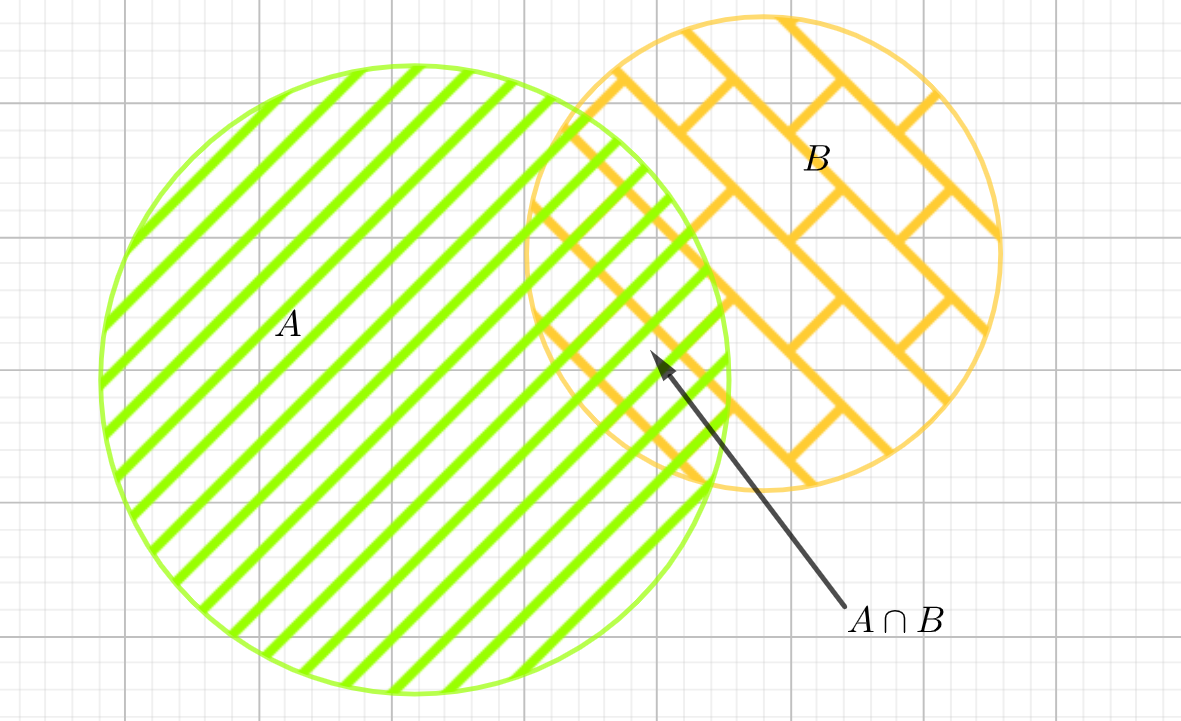
\includegraphics[height=30mm]{cond_prob}}
\hfill
\parbox[b][3 cm][t]{100mm}{
	Графически это означает, что, когда произошло событие $B$, мы оказались в круге $B$. Тогда формула  $\frac{\Pro(AB)}{\Pro(B)}$ есть просто вероятность попасть в $AB$.
}\\

Из определения следует так называемый <<Закон умножения вероятностей>>:
$$\Pro(A|B)\Pro(B)=\Pro(AB)$$

Легко проверяется, что $(B, \Ev_B, \Pro_B)$, где $\Ev_B = \Set{A \bigcap B}{A \in \Ev}$, так же является вероятностным пространством. \\
\begin{Wtf}
Зачем нужно требование $\Pro(B) > 0$, если можно в случае $\Pro(B) = 0$ доопределить условную вероятность нулем как вероятность при условии невозможного события?
При таком доопределении нарушится аксиома 3. вероятности $\Pro_B$, поскольку $\Pro_B(B)$ по доопределению будет равно $0$.
\end{Wtf}

\begin{Def}
События $A, B \in \Ev$ называются \underline{независимыми}, если $$\Pro(AB) = \Pro(A) \Pro(B)$$.
\end{Def}

Для независимых событий $$\Pro(A|B) = \frac{\Pro(A)\Pro(B)}{\Pro(B)} = \Pro(A)$$.\\
\begin{Ex}
Являются ли несовместные события ($AB = \varnothing$) независимыми? Нет, пусть  $A, B \in \Ev \colon \quad \Pro(A) > 0, \ \Pro(B) > 0$. Тогда $\Pro(AB) = \Pro(A)\Pro(B) = 0$, 
что является противоречием. По-простому, если произошло одно из несовместных событий, то второе уже не может произойти, и его условная веротяность равна 0, а не
вероятности самого события, что требуется для независимости.
\end{Ex}

Следующее определение обобщает понятие независимости на произвольное количество событий.
\begin{Def}
События $A_1, A_2, \dots, A_n$ называются \underline{независимыми в совокупности}, если 
$$\forall m = 2, \dots, n \quad \forall 1 \le j_1 < \ldots < j_m \le n \quad 
\Pro(\bigcap_{k=1}^{m}A_{j_k})=\prod_{k=1}^{m} \Pro(A_{j_k})$$
\end{Def}
\begin{Ex}
На примере тетраэдра Бернштейна можно убедиться в том, что попарной независимости событий недостаточно для независимости в совокупности. Рассмотри тетраэдр, у 
которого три стороны покрашены в красный, синий и зеленый, а четвертая содержит все три цвета. События \{выпадет красный\}=\{К\}, \{выпадет синий\}=\{С\}, \{выпадет зеленый\}=\{З\}
попарно независимы (например, вероятность события \{С\}$\bigcap$\{К\} равна веротяности выпадения четвертой грани, т. е. $\frac{1}{4}$, в то время как выпадения 
каждого цвета равна $\frac12$). Однако $\Pro$(\{С\}$\bigcap$ \{К\}$\bigcap$ \{З\}) = $\frac14 \not= (\frac12)^3$.
\end{Ex}
\newpage

\section{Формула полной веротяности. Формула Байеса}

\begin{Def}
$B_1, \ldots, B_n$ образуют \underline{полную группу}, если выполнены следующие условия:
	\begin{enumerate}
		\item $\Pro(B_i) > 0 \quad \forall i = 1, \ldots, n$
		\item $B_iB_j = \varnothing \quad (i \not= j)$
		\item $\bigcup\limits_{i=1}^nB_i = \Omega$
	\end{enumerate}
\end{Def}

\begin{Th}
Пусть $B_1, \ldots, B_n$ образуют полную группу. Вероятность события $A \in \Ev$ можно вычислить по \underline{формуле полной вероятности}:
$$\Pro(A) = \sum\limits_{i=1}^{n} \Pro(A|B_i)\Pro(B_i)$$
\end{Th}

\begin{Proof}
\\
$A=\bigcup\limits_{i=1}^{n}AB_i, \quad AB_i \bigcap AB_j = \varnothing \quad (i \not= j)$ \\
$\Pro(A) = \sum\limits_{i=1}^n \Pro(AB_i) = \sum\limits_{i=1}^{n} \Pro(A|B_i)\Pro(B_i)$ \\
Последний переход следует из  закона умножения вероятностей.
\end{Proof}
\\

Первое требование определения полной группы необходимо для возможности определить условную веротяность, второе позволяет 
разбить множество $A$ на непересекающиеся части. Третье требование, вообще говоря, можно ослабить, потребовав, чтобы $A \subseteq \bigcup\limits_{i=1}^nB_i$.
Доказательство при этом не изменится. 

\begin{Ex}
Проиллюстрировать формулу полной вероятности можно обычным экзаменом: $A$ - \{студент сдал экзамен\}, $B_i$ - \{студент попал к преподавателю $i$\}.
Как и в любой другой лотерее, можно оценить вероятность попадания к преподавателю $i$, то есть $\Pro(B_i)$, а трезво оценивая свои силы можно прикинуть 
и вероятность сдать тому или иному преподавателю $\Pro(A|B_i)$. Зная все вышеперечисленое, несложно по формуле вычислить вероятность успешной сдачи.
\end{Ex}
\\

Формула полной веротяности используется для вычисления априорной вероятности, т.е. вероятности события, которое  еще не произошло.
Пусть теперь \\$\Pro(A) > 0$. Тогда $\Pro(B_i|A)=\frac{\Pro(AB_i)}{\Pro(A)}$. Используя формулу полной вероятности, получаем \underline{формулу Байеса}:
$$\Pro(B_i|A)=\frac{\Pro(A|B_i)\Pro(B_i)}{\sum\limits_{j=1}^n\Pro(A|B_j)\Pro(B_j)}$$

Формула Байеса используется для вычисления апостериорной вероятности. То есть уже известно, что произошло некоторое событие $A$, и нужно вычислить вероятность
того, что произошло некоторое $B_i$. В примере с экзаменом, например, может быть известно, что студент не сдал экзамен, и хочется вычислить вероятность того, что он
сдавал Рублеву.

\section{Случайные величины}

\qquad Случайные события "--- это хорошо, но с события типа <<на монетке выпал герб>> плохо формализуемы, а мы хотим формальности и математичности. Поэтому вместо всяких событий хочется работать с числами. Вот этим и займемся. При рассмотрении случайных событий мы ввели вероятностное пространство, которе выглядит так:
$$(\Omega, \Ev, \Pro),$$
где $\Omega$ "--- множество элементарных событий, $\Ev$ "--- $\sigma$-алгебра подмножеств множества элементарных событий, а $\Pro$ "--- вероятность. Мы же будем рассамтривать теперь тройку
$$(\Real, \Bor, \Pro),$$
где $\Real$ "--- действительная прямая, $\Bor$ "--- Борелевская $\sigma$-алгебра, а $\Pro$ "--- вероятность. Поясним.

\begin{Def}
\underline{Борелевской $\sigma$-алгеброй} называется минимальная $\sigma$-алгебра, содержащая все открытые подмножества топологического пространства. Подмножества Борелевской $\sigma$-алгебры называются \underline{Борелевскими множествами}.
\end{Def}

\begin{Wtf}
Мы будем рассматривать только топологическое пространство $\Real$, так что это стремное словосочетание можно прямо 
сейчас забыть.
\end{Wtf}

\begin{Ex}
Покажем, что все <<хорошие>> множества являются Борелевскими.
\begin{enumerate}
\item Все открытые интревалы входят по определению.
\item Отрезок вида $[a, b]$ входит как $\overline{(-\infty, a) \bigcup (b, +\infty)}$.
\item Точка ходит как вырожденный отрезок $[a, a]$.
\item Счетное объединение таких множеств входит по поределению.
\end{enumerate}
\end{Ex}

Теперь формально введем понятие случайной величины (далее св).

\begin{Def}
Пусть $(\Omega, \Ev, \Pro)$ "--- вероятностное пространство. Тогда \underline{случайной величиной $\xi$} называется функция $\xi : \Omega \to \Real$, измеримая относительно $\Ev$ и $\Bor$. По-другому, $\xi$ "--- св, если
$$\forall B \in \Bor \quad \xi^{-1}(B) = \lbrace \omega : \xi(\omega) = B \rbrace \in \Ev$$.
\end{Def}

\begin{Wtf}
Таким финтом ушами мы, по сути, сопоставили каждому событию какое-то <<хорошее>> множество на числовой прямой, и можем рассамривать не вероятности событий, а вероятности подмножеств числовой прямой.
\end{Wtf}

Идем дальше в~сторону упрощения работы со случайностями. Вместо того чтобы рассматривать произвольные Борелевские множества, мы будем рассамтривать только множества вида $(-\infty, x)$. Действительно, интервал $(a, b)$ получается из~полупрямых так: $(a, b) = $ \textbf{ДИМА КАК ТУТ ПОЛУЧИТЬ ИНТЕРВАЛ ГЛАЗ ЗАМЫЛИЛСЯ?????!!} Таким образом, мы можем рассматривать св только на таких множествах. 

\begin{Def}
Рассмотрим вероятностное пространство $(\Omega, \Ev, \Pro)$ и определенную на нем св $\xi$. Тогда \underline{функцией распределения св $\xi$ $F_\xi(x)$} называется функция $F_\xi : \Real \to \Real$
$$F_\xi(x) = \Pro(\omega : \xi(\omega) < x) = \Pro(\xi < x)$$.
\end{Def}

Рассмотрим основные свойства функции распределения (далее фр):

\end{document}